\subsection{不良系统}

在适当缩放的系统上进行部分旋转的高斯消除可能是线性代数实际应用中最基本的算法。但它不是通用算法,也不能盲目使用。本节的目的是指出,在求解线性系统时,必须始终谨慎行事,因为有些系统对小扰动非常敏感,以至于无法放心使用数值技术。

\begin{example}
\label{example1.6.1}
考虑方程组:
$$
\begin{cases} 
.835x + .667y = .168, \\
.333x + .266y = .067
\end{cases}
$$
其精确解为$x=1$,$y=-1$。
若仅将$b_2=.067$轻微扰动为$\hat{b}_2=.066$,则精确解会显著变化为$\hat{x}=-666$,$\hat{y}=834$。
\end{example}
这是一个解对微小扰动极其敏感的方程组示例。这种敏感性是方程组本身固有的,并非由任何数值过程导致。因此,不能期望通过某种“数值技巧”来消除这种敏感性。如果精确解对微小扰动敏感,那么无论使用何种算法,计算出的解都不会不敏感。

\begin{bluebox}{病态线性系统}
当方程组的某些微小扰动可能导致精确解产生相对较大的变化时,该线性方程组被称为病态方程组;否则,该方程组被称为良态方程组。    
\end{bluebox}

对于包含两个未知数的$2\times2$方程组,很容易直观地理解病态的原因。在几何上,两个未知数的两个方程代表两条直线,交点就是系统的解。病态系统表示两条几乎平行的直线。

如果两条直线几乎平行,并且其中一条线仅稍微倾斜,则交点(即相关 $2\times2$ 线性系统的解)将发生巨大变化。

\begin{figure}
    \centering
    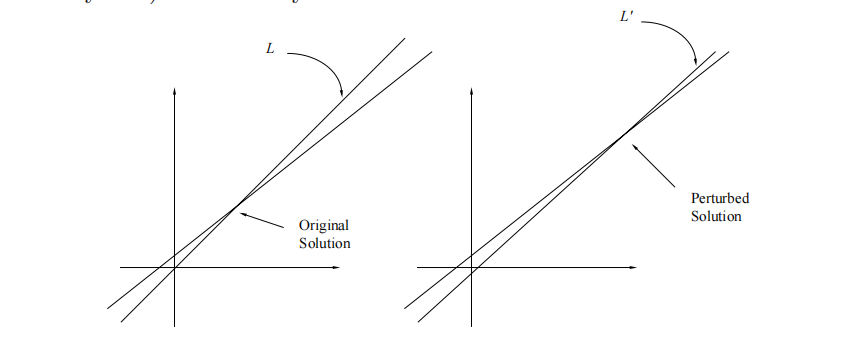
\includegraphics[width=0.8\textwidth]{images/fig1.6.1.png}
    \caption{1.6.1}
    \label{figure1.6.1}
\end{figure}

这在图\ref{figure1.6.1}中得到了说明,其中线 $L$ 被稍微扰动成为线 $L^{\prime}$ 。请注意这个小扰动如何导致交点发生较大变化。这正是例\ref{example1.6.1}中给出的系统的情况。一般来说,病态系统是那些代表几乎平行线、几乎平行平面以及这些概念的概括的系统。

因为舍入误差可以被视为对系统原始系数的扰动,所以即使在病态系统上使用一般良好的数值技术(缺乏精确的算术)也会带来产生无意义结果的风险。

在处理病态系统时,工程师或科学家经常面临比简单地尝试解决系统更基本(有时更令人不安)的问题。即使可以创造一个小奇迹,从而提取出精确的解决方案,科学家或工程师仍然可能得到一个无意义的解决方案,从而导致完全错误的结论。问题源于这样一个事实,即系数通常是凭经验获得的,因此只能在一定的公差范围内得知。对于病态系统,任何系数的微小不确定性都可能意味着解中可能存在极大的不确定性。这种巨大的不确定性甚至可能使精确的解决方案变得毫无用处。

\begin{example}
\label{example1.6.2}
假设方程组:
$$
\begin{cases} 
.835x + .667y = b_1, \\
.333x + .266y = b_2
\end{cases}
$$
中的$b_1$和$b_2$是实验结果,必须从测试仪器的刻度盘上读取。假设刻度盘的读数误差范围为$\pm .001$,且$b_1$和$b_2$的读数分别为$.168$和$.067$,这就构成了示例\ref{example1.6.1}中的病态方程组,并且已知该方程组的精确解为:
\begin{equation}
    (x,y) = (1,-1) \label{equation1.6.1}
\end{equation}
然而,由于刻度盘读数的微小不确定性,我们有:
\begin{equation}
.167 \leq b_1 \leq .169, \quad .066 \leq b_2 \leq .068 \label{equation1.6.2}    
\end{equation}
例如,这意味着读数$(b_1, b_2) = (.168, .067)$对应的解与读数$(b_1, b_2) = (.167, .068)$、$(b_1, b_2) = (.169, .066)$或落在范围(1.6.2)内的任何其他读数对应的解一样有效。对于读数$(b_1, b_2) = (.167, .068)$,精确解为:
\begin{equation}
    (x,y) = (934, -1169) \label{equation1.6.3}
\end{equation}
而对于另一个读数$(b_1, b_2) = (.169, .066)$,精确解为:
\begin{equation}
    (x,y) = (-932, 1167) \label{equation1.6.4}
\end{equation}

你愿意成为第一个乘坐设计中包含该问题解的飞机,或驾驶通过该问题解设计的桥梁的人吗?我不愿意!不确定性太大了。由于解\ref{equation1.6.1}、\ref{equation1.6.3}和\ref{equation1.6.4}中的任何一个都不比其他解更优,因此技术人员如何读取刻度盘上最后一位有效数字,可能会导致采用完全不同的设计方案。由于相关线性方程组的病态性质,飞机或桥梁的成功设计可能取决于运气,而非科学原理。
\end{example}

与其试图从病态方程组中提取精确解,工程师和科学家通常最好将时间和资源投入到重新设计相关实验或数据收集方法上,以避免产生病态方程组。

病态方程组还有另一个令人不安的方面,涉及学生所谓的“检验答案”——将计算出的解代入原方程组的左侧,看它与右侧的接近程度,从而判断解的正确性。更正式地说,若:

$$
x_c = \left(\begin{array}{llll} 
\xi_1 & \xi_2 & \cdots & \xi_n
\end{array}\right)
$$
是方程组:
$$
\begin{cases} 
a_{11}x_1 + a_{12}x_2 + \cdots + a_{1n}x_n = b_1, \\
a_{21}x_1 + a_{22}x_2 + \cdots + a_{2n}x_n = b_2, \\
\vdots \\
a_{n1}x_1 + a_{n2}x_2 + \cdots + a_{nn}x_n = b_n
\end{cases}
$$
的计算解,则称:
$$
r_i = a_{i1}\xi_1 + a_{i2}\xi_2 + \cdots + a_{in}\xi_n - b_i \quad (i = 1, 2, \cdots, n)
$$
为\textbf{残差}。假设你计算出一个解$x_c$,将其代入原方程组后发现所有残差都相对较小,这是否能保证$x_c$接近精确解?令人惊讶的是,当方程组是病态时,答案绝对是否定的!

\begin{example}
\label{example1.6.3}
对于示例\ref{example1.6.3}中的病态方程组,假设你计算出的解为
$$\xi_1 = -666, \quad \xi_2 = 834$$
若你试图通过将其代入原方程组来“检验误差”,使用精确算术计算可得残差:
$$
r_1 = .835\xi_1 + .667\xi_2 - .168 = 0
$$
$$
r_2 = .333\xi_1 + .266\xi_2 - .067 = -.001
$$
也就是说,计算解$(-666, 834)$精确满足第一个方程,且非常接近满足第二个方程。表面上看,这似乎表明计算解应该非常接近精确解。实际上,一个外行甚至可能被误导,认为计算解与精确解的误差在$\pm .001$范围内。显然,事实远非如此,因为精确解是
$$
x = 1, \quad y = -1
$$
对于第一次看到这种情况的学生来说,这总是一个冲击,因为它与新手的直觉相悖。不幸的是,许多学生毕业时仍然认为,通过将计算结果代入原方程,总能“检验”计算的准确性——很高兴你不属于这类学生。
\end{example}

这就引出了一个问题:“如何检验计算解的准确性?”幸运的是,若方程组是良态的,残差确实能更有效地衡量准确性。但这意味着你必须能够回答一些额外的问题,例如:如何预先判断给定的方程组是否是病态的?如何衡量线性方程组的病态程度?

一种确定病态程度的技术可能是:轻微扰动选定的系数,观察解的变化情况。若对某些系数的微小扰动导致解发生显著变化,则说明遇到了病态情况;若某个扰动未导致解发生较大变化,则无法得出结论——可能扰动的是错误的系数集。

通过对不同的系数集进行多次这样的实验,可以对病态程度有一个大致的了解(但不能保证准确)。这种方法成本高昂,且不太令人满意。但在开发出更复杂的工具之前,无法进一步深入讨论。

\begin{exercise}
\label{exercise1.6.1}
考虑示例\ref{example1.6.1}中的病态方程组:
$$
\begin{cases} 
.835x + .667y = .168, \\
.333x + .266y = .067
\end{cases}
$$
\begin{enumerate}[label=(\alph*)]
    \item 描述使用5位算术且不进行尺度变换时,求解该方程组的结果。\label{item1.6.1.a}
    \item 再次使用5位算术,但先对方程组进行行尺度变换,然后再尝试求解,描述这种方法的帮助程度。\label{item1.6.1.b}
    \item 现在使用6位算术且不进行尺度变换,求解该方程组,将结果与精确解进行比较。\label{item1.6.1.c}
    \item 使用6位算术,计算\ref{item1.6.1.c}中解的残差,并解释结果。\label{item1.6.1.d}
    \item 对于(c)中得到的同一个解,此次使用7位算术计算残差,并解释结果。\label{item1.6.1.e}
    \item 总结\ref{item1.6.1.a}到\ref{item1.6.1.e}中的要点,形成结论性陈述。
\end{enumerate}
\end{exercise}

\begin{exercise}
对上述练习\ref{exercise1.6.1}中的病态方程组进行扰动,形成以下方程组:
$$
\begin{cases} 
.835x + .667y = .166995, \\
.333x + .266y = .066995
\end{cases}
$$ 
\begin{enumerate}[label=(\alph*)]
    \item 确定该方程组的精确解,并将其与练习\ref{exercise1.6.1}中方程组的精确解进行比较。\label{item1.6.2.a}
    \item 根据\ref{item1.6.2.a}的结果,就病态方程组的解是否必然会因原方程组的每次扰动而发生显著变化这一问题,形成陈述。
\end{enumerate}
\end{exercise}

\begin{exercise}
考虑由以下两个方程的图像确定的两条直线:
$$
\begin{cases} 
.835x + .667y = .168, \\
.333x + .266y = .067
\end{cases}
$$
\begin{enumerate}[label=(\alph*)]
    \item 使用5位算术计算每条直线的斜率,然后使用6位算术重复计算,在每种情况下,在坐标系中绘制图像。
    \item 通过图形说明,为什么对其中任何一条直线的微小扰动都可能导致解发生较大变化。
    \item 用几何术语描述方程组为最优良态时必须满足的条件。
\end{enumerate}
\end{exercise}